\documentclass[a4paper,12pt]{article}

\usepackage{amsmath}
\usepackage{hyperref}
\usepackage{graphicx}
\usepackage[margin=1in]{geometry}

\usepackage[T1]{fontenc}
\usepackage{tgschola}

\title{
  \centering
  \flushright\footnotesize\today\\
  \centering
  \rule{\textwidth}{1.6pt}\vspace*{-\baselineskip}\vspace*{2pt}
  \rule{\textwidth}{0.4pt}\\[\baselineskip]
  {\Huge \scshape
    Controlling a Rocket\\[10pt]
  }
  \rule{\textwidth}{0.4pt}\vspace*{-\baselineskip}\vspace*{3.2pt}
  \rule{\textwidth}{1.6pt}\\[0.5\baselineskip]
  {\scshape \large
    ENEL430 Assignment Two\\
  }
  \vspace*{1.5\baselineskip}
  {\Large
    {\scshape Wim Looman} (\emph{92692734})\\
    \href{mailto:wgl18@uclive.ac.nz}{wgl18@uclive.ac.nz}\\
  }
}

\author{
  \vspace*{-2\baselineskip}
}

\date{
  \vspace*{-2\baselineskip}
}

\setlength{\parskip}{10pt}
\setlength{\parindent}{0pt}

\begin{document}

  \maketitle

  \section{Introduction}

    In order to correctly design controllers for complex systems such as a
    rocket an accurate model must be created.  One major method for creating
    this model is known as System Identification.  System Identification is
    about utilising statistical methods to build mathematical models of
    dynamical systems from measured data.

    The system used in this report consisted of a vertical wind tunnel
    containing a 1.4m long rocket suspended by a string.  This allowed the
    rocket to freely rotate with negligible extraneous damping while wind flowed
    past at up to 110 km/hr.

    The form of the model in relation to the roll rate ($\dot\theta$) was found to be:

    \begin{equation}
      \ddot\theta = -a_\text{final}\dot\theta + b_\text{final} u_\text{f} + f_0
    \end{equation}

    With the measured fin angle ($u_\text{f}$) obeying a non-linear function ($F$) in
    terms of the commanded fin angle ($u_\text{cmd}$).

    \begin{equation}
      u_\text{f} = F\left(u_\text{cmd}\right)
    \end{equation}

    \begin{equation}
      u_\text{cmd} = k_p \left(R_\theta - \theta\right) + k_d \left(-\dot\theta\right)
    \end{equation}

    $R_\theta$ is the set point for the controller.

    This can be converted into a more detailed model:

    \begin{align}
      \ddot\theta &= -a_\text{final}\dot\theta + b_\text{final} y_1 + f_0 \\
      \dot u_\text{cmd} &= -k_p \dot\theta - k_d \ddot\theta \\
      \dot y_1 &= y_2 \\
      \dot y_2 &= -C_1 y_2 - K_1 y_1 + C_2 \left(-k_p \dot\theta - k_d \ddot\theta \right) + K_2 \left( k_p \left( R_\theta - \theta \right) - k_d r \right)
    \end{align}

    With this model three controllers were designed.  The first was designed
    with a relatively high $k_p$ gain and low $k_d$ gain in order to induce
    oscillations.  The second was aimed at an optimal response and the third was
    another attempt at an optimal response with higher gains.


  \section{Results and Discussion}

    The three controllers were designed using a provided model with $C_1 =
    6.3965$, $C_2 = 6.3141$, $K_1 = 1.2494$, $K_2 = 1.7439$ and $\beta =
    2.0193$.  The values found were:

    {
      \centering
      \begin{tabular}{l||r|r}
        \textbf{Controller} & $\boldsymbol{k_p}$ & $\boldsymbol{k_d}$ \\
        \hline
        One & 1.00 & 0.20 \\
        Two & 0.37 & 0.48 \\
        Three & 0.80 & 0.60 \\
      \end{tabular}
    }

    Figure \ref{fig:one} shows the response of the first controller.  The model
    appears to have much less damping than the measured data.  This is likely
    partly from saturation of the fin angle.  The controller on the rocket
    limits the fin angle to $\pm 20$ degrees, viewing the output of the fin
    angle it can be seen that these limits are being hit a lot while this
    controller was running.

    Figure \ref{fig:two} shows the response of the second controller, this is
    much better than the first.  In fact the error in the model is less than 2\%
    compared to over 20\% for the first model.

    Figure \ref{fig:three} shows the response of the third controller.  This
    is not as good as the second controller -- at around 6\% error -- but it is
    still much better than the first one.  The rise time on this controller was
    quite a bit better than the second controller however, although not as much
    better as the models were predicting.

    The fact that all models had faster responses than the measured data
    indicates that the real rocket had higher damping than the models were
    using.  An attempt at finding better $a_\text{final}$ and $b_\text{final}$
    values was performed using a brute force system based off the first
    controllers response.  This resulted in values of $a_\text{final} = 0.89$
    and $b_\text{final} = 2.2$ with the associated model responses shown dashed
    on the figures.  The errors in the three model responses with these values
    was 6\%, 11\% and 3\%.

    \begin{figure*}[p]
      \centering
      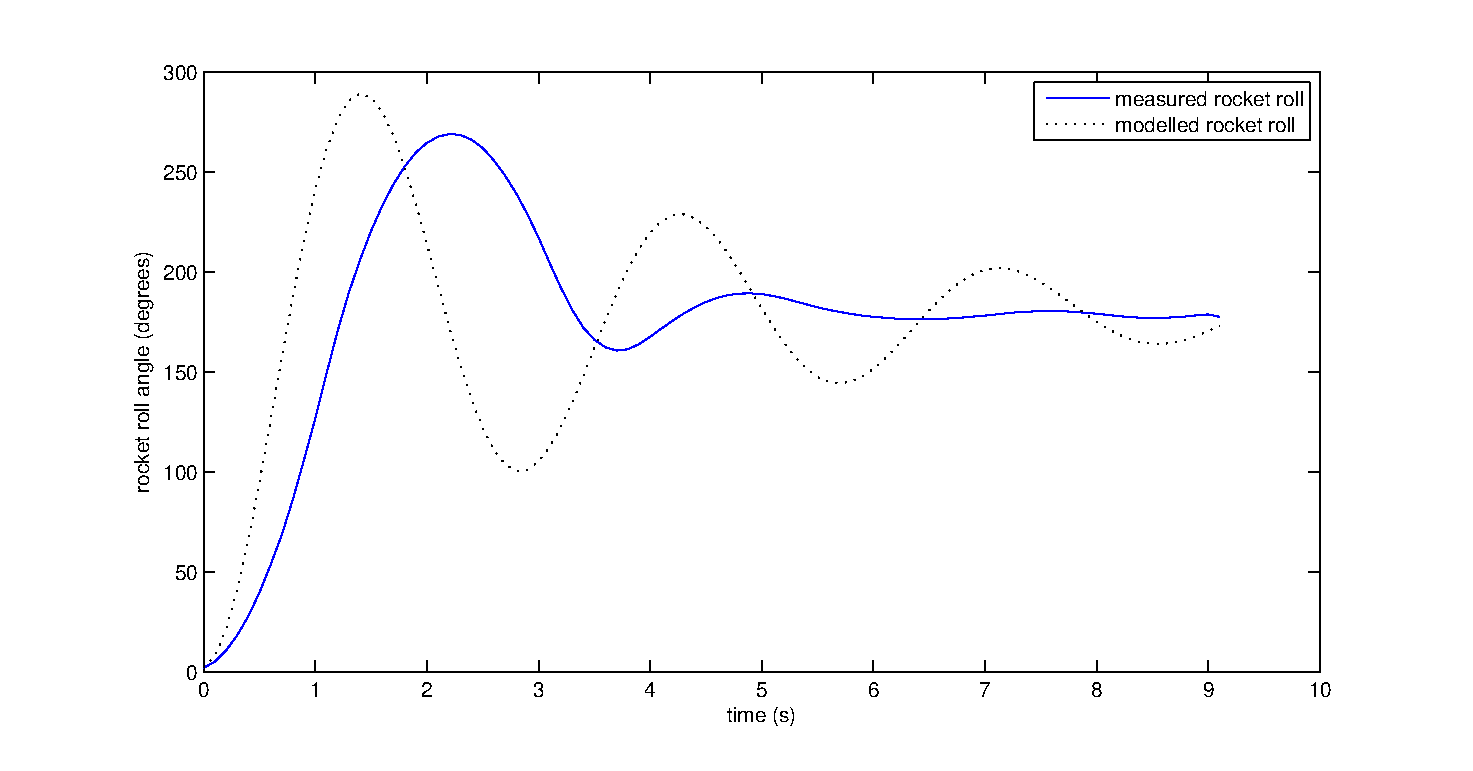
\includegraphics[height=0.25\textheight]{one}
      \caption{Response of first controller}
      \label{fig:one}
    \end{figure*}

    \begin{figure*}[p]
      \centering
      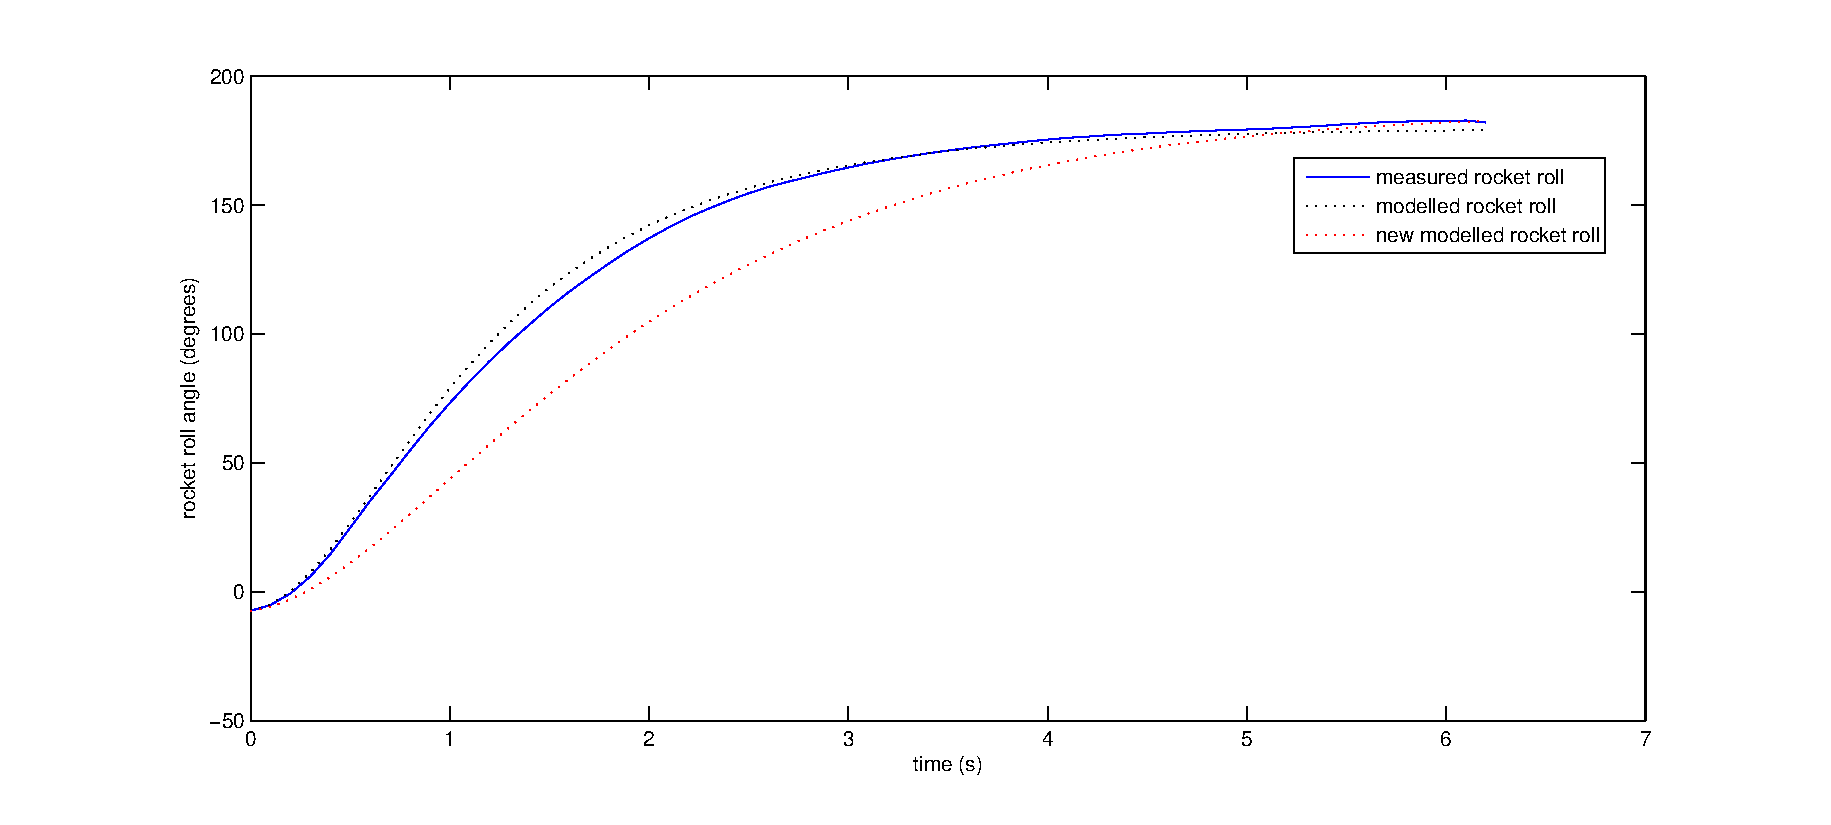
\includegraphics[height=0.25\textheight]{two}
      \caption{Response of second controller}
      \label{fig:two}
    \end{figure*}

    \begin{figure*}[p]
      \centering
      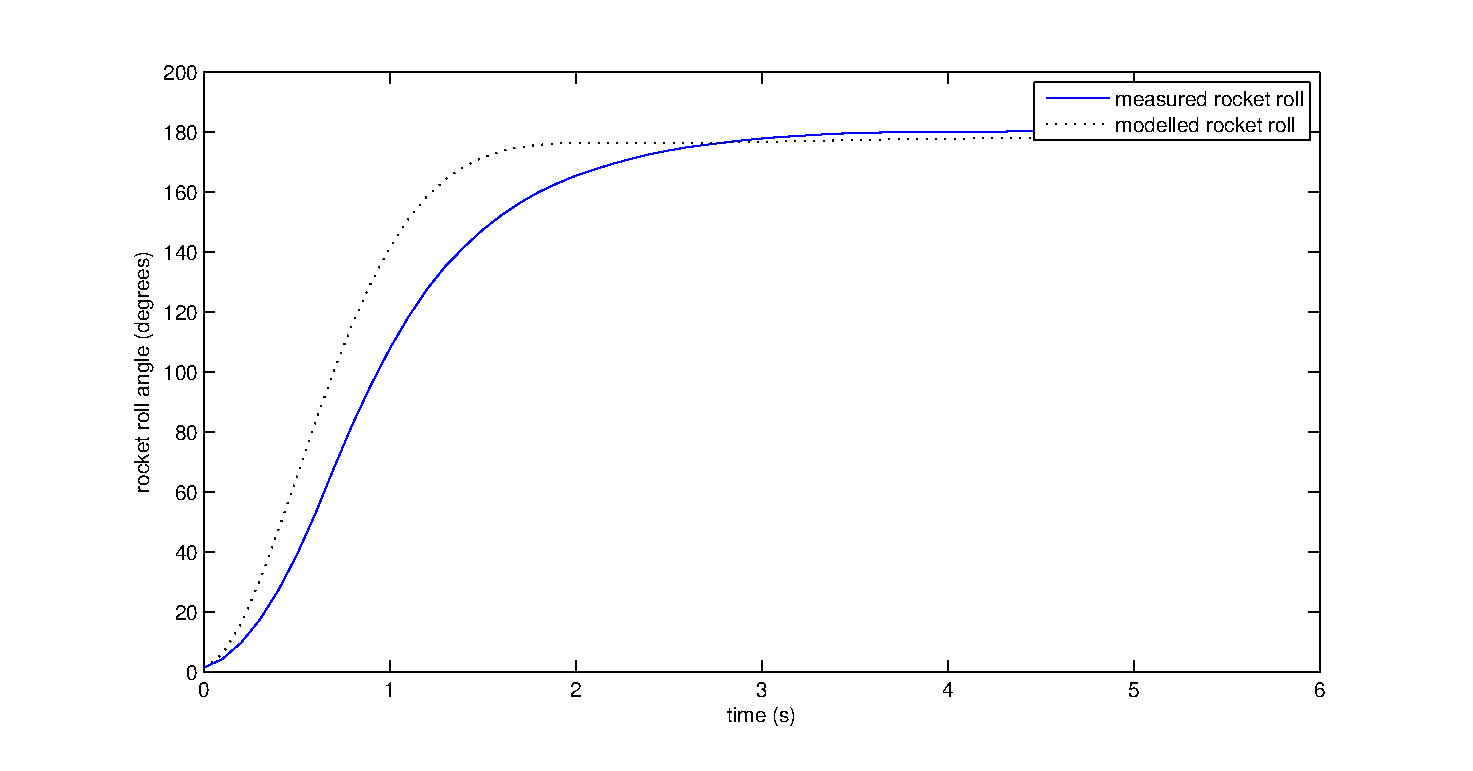
\includegraphics[height=0.25\textheight]{three}
      \caption{Response of third controller}
      \label{fig:three}
    \end{figure*}

\end{document}
